\documentclass[
  DIV=11,                 %% Satzspiegelkonstruktion, siehe KOMA-Script Anleitung
  fontsize=11pt,          %% Text in Schriftgrad 11pt
  BCOR=10mm,              %% Bindekorrektur, Klemmbindung verbraucht ca. 10mm
  captions=tableheading,  %% Tabellen haben eine Überschrift!
  headinclude=true,       %% Kopfzeile wird zum Satzspiegel gerechnet
  footinclude=false,      %% Fußzeile zählt zum Seitenrand (weil nur Seitenzahl in Fußzeile)
  headings=normal,        %% Überschriften etwas verkleinern (auf LARGE)
  numbers=noenddot,       %% kein Endpunkt bei Gliederungsnummerierung
  listof=flat,            %% Verzeichnisse der Gleitumgebungen nicht einrücken
  %draft,                  %% Draftmodus, keine Bilder/Farben
]{scrreprt}                


\usepackage[T1]{fontenc}      %% europäische Zeichensätze
\usepackage[utf8]{inputenc}   %% UTF-8 Kodierung, direkte Eingabe von Umlauten 
\usepackage[ngerman]{babel}   %% deutsche Anpassungen

%% Mathe-Pakete
%% ------------------------------------------------------------------------------
\usepackage{amsmath}       %% Matheumgebung
%\usepackage{amsfonts}     %% zusätzliche Mathe Schriften
%\usepackage{amssymb}      %% zusätzliche Symbole


%% noch mehr Symbole bei Bedarf
%% ------------------------------------------------------------------------------
\usepackage{latexsym}      %% zusätzliche Symbole
\usepackage{textcomp}      %% zusätzliche Symbole
\usepackage{eurosym}       %% Euro Symbol


\usepackage{siunitx}       %% richtige Schreibweise für SI Einheiten

\usepackage{setspace}      %% Zeilenabstand anpassen


%%------------------------------------------------------------------------------
%% Schriftauswahl
%%------------------------------------------------------------------------------
%\usepackage{lmodern}                 %% Latin Modern

%\usepackage{mathpazo}                %% Palatino

\usepackage[charter]{mathdesign}      %% Charter

%% für Charter und Palatino Zeilenabstand leicht erhöhen (1.05 bis 1.08)
\setstretch{1.08}            %% Einstellung schriftabhängig, für Latin Modern deaktivieren!

%% Bera Sans als serifenlose Schrift
\usepackage{berasans}

%% Bera Mono als monospaced Schrift (für fette Keywords in Listings)
\usepackage[scaled]{beramono}
%%------------------------------------------------------------------------------


%% Satzspiegel nach Schriftauswahl neu berechnen
\KOMAoptions{DIV=current}

%% Überschriften für alle Gliederungsebenen in fett und der gleichen
%% Schriftart wie den Standardtext setzen
\setkomafont{disposition}{\normalfont\bfseries}


%% Anpassung von Kopf- und Fußzeilen
%%------------------------------------------------------------------------------
\usepackage{scrpage2}        %% KOMA-Script Erweiterung für Kopf-/Fußzeilen
\pagestyle{scrheadings}      %% Seitenstil scrheadings verwenden
\clearscrheadfoot            %% alle Felder in Kopf- und Fußzeile löschen
\automark[chapter]{chapter}  %% Kopfzeile: Kapitelname außen


%% optischer Randausgleich
\usepackage{microtype}

%% korrektes Leerzeichen nach Makro
\usepackage{xspace}

%% einheitliche Anführungszeichen festlegen
%% Aufruf: \enquote{was in Anführungszeichen stehen soll}
\usepackage[
  babel,
  %german=guillemets,  %% spitze Klammern
  german=quotes,       %% normale Anführungszeichen
]{csquotes}


%% erweiterte Farbmöglichkeiten mit xcolor
%% Option [table] lädt das Package colortbl nach
\usepackage[table]{xcolor}

%% Abbildungen einbinden
\usepackage{graphicx}
\usepackage{wrapfig}

%% Zeilenabstand in Auflistungen verringern
%% Aufruf mit {enumerate*} bzw. {itemize*} 
\usepackage{mdwlist}


%% Tabellen
%% ------------------------------------------------------------------------------
\usepackage{booktabs}    %% für bessere Linien 	top-/mid-/bottomrule	
\usepackage{tabularx}    %% erweiterte Tabellendefinitionen 
\usepackage{longtable}  %% Lange Tabellen über mehr als eine Seite
\usepackage[bottom]{footmisc}  %% verhindert, dass Bilder unter Fußnoten rutschen


%% Tabellen- und Bildbeschreibungen anpassen
%% ------------------------------------------------------------------------------
\setlength\abovecaptionskip{2pt}    %% Abstand der Beschreibung zum Objekt
%% Schrift für Label und Beschreibungstext wie für normalen Text
\setkomafont{captionlabel}{\small\normalfont\bfseries}
\setkomafont{caption}{\small\normalfont}


%% Verarbeitung bibliografischer Daten mit Biblatex
%% Über Option  backend  entweder biber oder bibtex verwenden
%% Im Editor für Bib(la)tex folgenden Befehl eintragen:
%%     biber %    oder    bibtex % 
%% ------------------------------------------------------------------------------
\usepackage[
  style=numeric,   %% numerischer Stil
  isbn=false,      %% keine ISBN ausgeben
  url=false,       %% keine URL ausgeben
  backend=biber,   %% entweder biber zur Verarbeitung von Literaturverweisen 
  %backend=bibtex,   %% oder bibtex (veraltet, kann keine Umlaute verarbeiten) 
  %backref,         %% Rückverweise auf Zitate
]{biblatex}


%% Darstellung im Literaturverzeichnis mit biblatex auf Name, Vorname umstellen
%%------------------------------------------------------------------------------
\DeclareNameFormat{default}{%
\usebibmacro{name:last-first}{#1}{#3}{#5}{#7}%
\usebibmacro{name:andothers}}


%% Quellcode anzeigen, Standardeinstellungen
%% ------------------------------------------------------------------------------
\usepackage{listings}
\renewcommand{\lstlistlistingname}{Quelltextverzeichnis}    %% Umbenennen
\lstset{
  float=tb,
  captionpos=t,
%   basicstyle=\small\ttfamily,
  basicstyle=\tiny\ttfamily,
  keywordstyle=\bfseries,
  commentstyle=\ttfamily,
  columns=fixed,
  tabsize=2,
  %frame=single,      %% einfache Linie als Umrandung
  framerule=0.1pt,
  extendedchars=true,
  showspaces=false,
  showstringspaces=false,
  numbers=left,
  numberstyle=\sffamily\tiny,
  breaklines=true,
%  backgroundcolor=\color{black!10},      %% Hintergrundfarbe helles Grau
  breakautoindent=true,
  belowskip=2ex,
  literate=%         %% Umlaute wg. utf8 ersetzen z.B.  ü durch \"u
    {Ö}{{\"O}}1 {Ä}{{\"A}}1 {Ü}{{\"U}}1
    {ß}{{\ss}}1 {ü}{{\"u}}1 {ä}{{\"a}}1 {ö}{{\"o}}1
}


%% Listings-Umgebung für Fortan77 definieren, nur Inline Code!
%% Aufruf mit:
%% \begin{fortran}{Beschriftungstext}{lst:labelname}
%%   hier der FORTAN-CODE
%% \end{fortran}
%%--------------------------------------------------------------
\lstnewenvironment{fortran}[2]{%
  \lstset{caption=#1,label=#2,language={[77]Fortran}}
}
{}

\lstnewenvironment{dict}[2]{%
  \lstset{caption=#1,label=#2,language={C++}}
}
{}
%%--------------------------------------------------------------


%% Warnungen von KOMA-Script für Entwickler umgehen
\usepackage{scrhack}

%% Blindtext
\usepackage{blindtext}


%% Verweise/Links für PDF, möglichst zuletzt laden!
%-----------------------------------------------------------------------------
\usepackage[
  pdfborder={0 0 0},
  %colorlinks=true,    %% farbige Links am Bildschirm, false oder deaktiviert für Ausdruck
  pdfstartview=FitV,   %% wie soll Viewer starten?
  linkcolor=blue,      %% Farbe für Querverweise
  citecolor=blue,      %% Farbe für Zitierungen
  urlcolor=blue,       %% Farbe für Links
  bookmarks=true,      %% Lesezeichen im PDF
  bookmarksnumbered,   %% nummerierte Kapitel
  plainpages=false,
]{hyperref}


%% das offizelle Euro Symbol verwenden, muss nach hyperref stehen!
\let\texteuro\euro

%
%\documentclass[a4paper,11pt]{article}
%\usepackage[T1]{fontenc}
%\usepackage[utf8]{inputenc}
%\usepackage{lmodern}
%\usepackage{ngerman}
\usepackage{hyperref, wasysym}
\usepackage{todonotes}
%\usepackage{geometry}
%
%\geometry{verbose,a4paper,tmargin=25mm,bmargin=25mm,lmargin=15mm,rmargin=20mm}

\title{\textit{FancyFOAM}\\Der Versuch einer umfassenden Dokumentation von \textsc{OpenFOAM}}

\author{Aljoscha N. Sander}

%% Silbentrennungen für bestimmte Wörter festlegen, kann auch
%% in eine Datei ausgelagert und mittels \input eingebunden werden.
\hyphenation{Recht-schreib-fehler}


%%---------------------------------------------------------
%% Hier beginnt das Dokument
%%---------------------------------------------------------
\begin{document}

%% erstmal ohne Seitennummern
%%%---------------------------------------------------
%% Titelseite für Studienarbeiten,
%% ensprechende Texte bei Bedarf ändern/löschen 
%%---------------------------------------------------

%% Warnung "destination with the same identifier (name{page.1})"
%% unterdrücken, versursacht durch hyperref Paket
\pagenumbering{alph}
%%---------------------------------------------------

\begin{titlepage}
  \enlargethispage{2.5cm}   %% Textbereich etwas nach unten vergrößern
  \begin{center}            %% Titelseite zentriert
    
\includegraphics[scale=0.4]{Abbildungen/logohsb.pdf}\\  %% Logo der Hochschule einbinden
    Fakultät 5 -- Natur und Technik
    
    \vspace{12ex}                          %% Abstand
    \huge{\textbf{\titel}}\\[7ex]          %% Titel der Arbeit einfügen
    \LARGE{\textbf{\art}}\\[1.5ex]         %% Bachelor- oder Masterarbeit oder ...
    \Large{im Fachgebiet {\fachgebiet}}    %% Fachgebiet innerhalb der Studienganges
    \normalsize
    \vfill                                 %% Abstand nach unten auffüllen

    \begin{tabularx}{\textwidth}{>{\raggedleft\arraybackslash}X>{\raggedright\arraybackslash}X}
      vorgelegt von:     & \autor\\[1.2ex]
      Matrikel Nr.:      & \matrikel\\[1.2ex]
      Fachrichtung:      & \fachrichtung\\[1.2ex]
      Erstprüfer:        & \erstpruefer\\[1.2ex]
      Zweitprüfer:       & \zweitpruefer\\[1.2ex]
      Datum der Abgabe:  & \abgabedatum\\[2ex]
    \end{tabularx}
  
  \end{center}
\end{titlepage}
        %% Deckblatt
%%%-------------------------------------------
%% Erklärung und Sperrvermerk
%%-------------------------------------------
\thispagestyle{plain}       %% Keine Kopf- und Fußzeile

\vspace{5ex}
\minisec{\LARGE{Erklärung}}
\vspace{3ex}
Hiermit erkläre ich, dass ich die vorliegende Arbeit selbstständig angefertigt habe. Es wurden nur die in der Arbeit ausdrücklich genannten Quellen und Hilfsmittel benutzt. Wörtlich oder sinngemäß übernommenes Gedankengut habe ich als solches kenntlich gemacht.
\vspace{5ex}

\begin{tabular}[h]{lp{2cm}p{5.5cm}}
  \centering
  Bremen, \hspace{2.5cm} &  &  \\
  \cline{1-1} \cline{3-3}
  \sffamily\scriptsize{Ort, Datum}  &  &  \sffamily\scriptsize{Unterschrift}\\
\end{tabular}

\vfill

%% Sperrvermerk, falls nötig
\minisec{\LARGE{Sperrvermerk}}
\vspace{3ex}
%% Text anpassen, eventuell mit Prüfer absprechen
Die vorliegende \art ist mit einem Sperrvermerk versehen und wird ausschließlich zu Prüfungszwecken an der Fachrichtung \textit{\fachrichtung} der Hochschule Bremen vorgelegt. Jede Einsichtnahme und Veröffentlichung -- auch von Teilen der Arbeit -- bedarf der vorherigen Zustimmung durch den Verfasser und der Firma Deutsches Forschungszentrum für künstliche Intelligenz, Bremen, Deutschland.

\vspace{5ex}

\begin{tabular}[h]{lp{2cm}p{5.5cm}}
  \centering
  Bremen, \hspace{2.5cm} &  &  \\
  \cline{1-1} \cline{3-3}
  \sffamily\scriptsize{Ort, Datum}  &  &  \sffamily\scriptsize{Unterschrift}\\
\end{tabular}
        %% Erklärung, Sperrvermerk

\maketitle

\clearpage                     %% Seite beenden und ausgeben

%%---------------------------------------------------------
%% Verzeichnisse einfügen
%%---------------------------------------------------------
\ofoot[\pagemark]{\pagemark}   %% ab hier Seitenzahlen in Fußzeile anzeigen
\pagenumbering{roman}          %% römische (kleine) Seitenzahlen vor dem Hauptteil

\tableofcontents               %% Inhaltsverzeichnis einfügen

\listoffigures                 %% Abbildungsverzeichnis bei Bedarf einfügen

\listoftables                  %% Tabellenverzeichnis bei Bedarf einfügen

\lstlistoflistings             %% Quelltextverzeichnis bei Bedarf einfügen

%% Eintr�ge f�r Abk�rzungsverzeichnis
%% nur verwendetete fachbezogene Abk�rzungen eintragen!
\chapter*{Abkuerzungen}

\begin{longtable}[l]{@{}p{50pt} p{200pt}}
IMO     &  International Maritime Organization\\
MDOF    &  Multiple degree-of-freedom\\
SDOF    &  Single degree-of-freedom\\
SWATH   &  Small Waterplane Area Twin Hull\\
\end{longtable}



%% Eintr�ge f�r Symbolverzeichnis
\chapter*{Symbolverzeichnis}

\begin{longtable}[l]{@{}ccp{300pt}}
\textbf{Symbol}	& \textbf{Einheit} & \textbf{Beschreibung} \\
$L$	 	& \si{\meter}					& Laenge\\
$A$		& \si{\milli\meter\squared}		& Flaeche\\
\end{longtable}


\clearpage                     %% Seite beenden und ausgeben

\begin{abstract}
Dokumentation der wichtigsten Eigenschaften von OpenFOAM. 
\end{abstract}

\newpage


%%---------------------------------------------------------
%% Hier beginnt der Haupteil 
%%---------------------------------------------------------
\pagenumbering{arabic}    %% arabische Seitenzahlen im Hauptteil
\ohead[]{\rightmark}      %% Kopfzeile mit Kapitelname (nicht auf Kapitelanfangsseiten)

%%---------------------------------------------------------
%% Die einzelnen Kapitel einbinden
%%---------------------------------------------------------
\chapter{Linux}

OpenFOAM ist grundsätzlich auf verschiedenen Betriebssystemen lauffähig. Innerhalb dieses Dokuments wird jedoch davon ausgegangen, dass OpenFOAM unter einem modernen UNIX Betriebssystem (streng genommen sollte dadurch MAC OS X davon ausgenommen werden, da MAC grundlegende POSIX-Richtlinien links liegen lässt und (mal wieder) den armen Nutzern vorgaukelt es würde alles viel besser machen. Was in diesem Fall nicht stimmt, da es durch die POSIX-Violation erheblichen Aufwand erfordert OpenFOAM unter MAC zum laufen zu bekommen. Sollte der Leser aber unter MAC OS X arbeiten, gehe ich davon aus, dass er entweder eine Virtuelle Maschine mit einem anständigen Betriebssystem zur Verfügung hat oder so gut ist, dass er OpenFOAM gepatcht und von Hand kompiliert hat. Sollte letzteres der Fall sein, darf der Leser getrost das folgende Kapitel überspringen) wie bspw. Linux läuft. 
\\
\section{Was, Warum und Wer ist Linux}
Linux ist streng genommen zunächst mal eine Software, welche in der Lage ist mit Hardware zu kommunizieren und Kommunikationskanäle zwischen den verschiedenen Hardwarekomponenten eines Computers zur Verfügung zu stellt. Linux stellt somit den elementaren Teil eines Betriebssystems dar (für Leser die \underline{nicht} wissen, wass was ein Betriebssystem ist; Wikipedia ist treuer als so manches Haustier und geduldiger als so manche Ehefrau... ;-) ). In Kombination mit viel anderer Software (welche gemeinhin als Distribution bezeichnet wird) stellt es ein freies \footnote{frei nicht immer im Sinne von kostenlos. Frei in dem Sinn, dass der Quellcode frei Verfügbar ist und jeder diesen Quellcode nutzen darf (durchaus auch zur kommerziellen Nutzung).} Betriebssystem zur Verfügung. Populäre Distributionen sind u.A. Ubuntu, Debian, OpenSUSE, Fedora, Arch Linux, Cent OS, uvm. Diesen Distrubtionen ist gemein, dass Sie alle im Kern auf Linux basieren und dem POSIX-Standard genügen.

Die vorhandenen Linuxdistributionen bietet den unschlagbaren Vorteil, dass es von vielen Nerds, verteilt über den ganzen Globus \footnote{Fun Fact: und darüber hinaus; die Laptops der ISS-Besatzung laufen auf Debian; die Rechner auf Arktisforschungsstationen und Tiefseerobotern ebenfalls. Linux IST überall.} verteilt entwickelt wird. Wobei die verschiedenen Distributionen verschiedene Anwender im Fokus haben. Allen gemein ist es jedoch, dass es äußerst einfach ist neue Software auf Linux zum laufen zu bringen. Was wiederum der freien Zugänglichkeit der Software geschuldet ist. Anyways, es gibt viele, viele weitere Gründe warum Linux wunderbar und fabelhaft ist, sicherlich ebenbürtig viele Gründe die gegen das Betriebssystem sprechen \footnote{u.A.: http://ubuntuforums.org/showthread.php?t=1852199 , http://linuxhaters.blogspot.de/}. 
\\
Der Grund warum dieses Dokument mit einem Kapitel über Linux beginnt ist einfach: OpenFOAM ist genau genommen kein einzelnes Programm, sondern eine gigantische Bibliothek (auch als Framework bezeichnet) an Software, deren Gemeinsamkeit darin besteht, das sie alle über eine Konsole bedient werden. Linux stellt eine POSIX-konforme Konsolenumgebung zur Verfügung, welche, unter den richtigen Umständen und mit dem richtigen Wissen genutzt, äußerst effizientes Arbeiten erlaubt. Dazu folgen im nächsten Kapitel die wichtigsten Befehle.

\section{Die wichtigsten Konsolenbefehle}

\begin{table}[htb]
  \centering
%  \begin{tabular}{@{}*{2}{l}@{}} 
  \begin{tabular}{m{3cm}m{9cm}} 
  \toprule
    	Befehl & Aktion \\
  \midrule
  
    	man BEFEHL & Der wichtigste Befehl überhaupt; öffnet ein Handbuch mit Erklärungen und Beispielen zum Befehl BEFEHL \\
    	
    	cd PFAD & change directory. Wechselt in das angegebene Verzeichnis \\
    	
    	cp [-rv] QUELLE ZIEL & kopiert QUELLE nach ZIEL. vorsicht, überschreibt auch Dateien. Das kopieren von Verzeichnissen ist nur mit der Option -r möglich \\
    	
    	rm [-rfv] DATE1 VERZEICHNIS1 ... & löscht die/das DATEI1/VERZEICHNIS1 \footnote{ACHTUNG: löschen heißt \underline{\textbf{NICHT}} in den Papierkorb verschieben. Löschen heisst töten, umbringen, über den Jordan, kurz: es ist unwiederruflich.} \footnote{naja fast: mein Stundenlohn beträgt 150 € / h} \\
    	
    	cat DATEI & gibt den gesamten Inhalt von DATEI auf der Konsole aus. \\
    	
    	less DATEI & öffnet die Datei DATEI und ermöglicht ein skrollen, springen und durchsuchen der Datei mittels Tastenkombinationen. \\
    	
    	tail [-fn ZAHL] DATEI & gibt den letzten Teil einer Datei aus oder gibt kontinuierlich aus was in die Datei DATEI geschrieben wird. \\
    	
    	BEFEHL1 | BEFEHL2 & das Sonderzeichen | (auch als pipe bezeichnet) verknüpft zwei Befehl miteinander, so dass der output des ersten Befehls als input für den zweiten Befehl genutzt werden kann. \\
    	
    	grep [-Rinl] SCHLAGWORT VERZEICHNIS/DATEI & durchsucht die Datei DATEI oder alle Dateien im Verzeichnis VERZEICHNIS nach SCHLAGWORT. \\ 
    	
    	find VERZEICHNIS -iname NAME -type TYP -exec BEFEHL & Durchsucht VERZEICHNIS nach Dateien des Typs TYP mit dem namen NAME und führt (wenn so spezifiziert) den befehl BEFEHL aus. \\
		
  \bottomrule
  
     
  \end{tabular}
  \caption[Konsolenbefehle]{Konsolenbefehle}
  \label{tab:befehle} 
\end{table}

\newpage
\chapter{Strömungsmechanik}

\begin{itemize}
	\item Impulsgleichung
	\item Energiegleichung
	\item Masseerhaltung
	\item Impulsgleichung für inkompressible, newtonsche Fluide (N-S Gleichung)
	\item Impulsgleichung für kompressible, newtonsche Fluide 
\end{itemize}

Wir gehen zunächst von einem inkompressiblen, newtonschen Medium für das die Kontinuumshypothese gilt aus. Dadurch wird die Impulsgleichung zur Navier-Stokes-Gleichung (\autoref{eq:ns}):

\begin{equation}
	\label{eq:ns}
	\frac{\partial u_{i}}{\partial t} + u_{j} \frac{u_{i}}{x_{j}} = - \frac{ \frac{p}{\rho} + g k}{\partial x_{i}} + \nu \frac{\partial^{2} u_{i}}{\partial u_{j}^{2}}
\end{equation}

Durch die Inkompressibilität vereinfachst sich die Kontiuumsgleichung zu \autoref{eq:konti}:

\begin{equation}
	\label{eq:konti}
	\frac{\partial u_{i}}{\partial x_{i}} = 0
\end{equation}

Der erste Term von \autoref{eq:ns}, $ \frac{\partial u_{i}}{\partial t} $ wird als instationärer Term bezeichnet, er repräsentiert den Einfluss der Änderung des Impulses über die Zeit. Der zweite Term $ u_{j} \frac{u_{i}}{x_{j}} $, auch als konvektiver Term bezeichnet, beschreibt die Impulstransport aufgrund von Geschwindigkeitsänderungen. Dieser Term ist nichtlinear. 
Der dritte Term $ - \frac{ \frac{p}{\rho} + g k}{\partial x_{i}} $ ist der Druckgradient. In OpenFOAM wird der Druckgradient mit weiteren äußeren Kräften, wie z.B. der Gravitation (bei mehrphasigen Systemen) oder elektromagnetischen Kräften zusammengefasst. 
Der letzte Term $ \nu \frac{\partial^{2} u_{i}}{\partial u_{j}^{2}} $, auch als diffusiver Term bezeichnet. 

\newpage
\chapter{Turbulenz}
	\section{RANS}
	\section{LES/DES}
\newpage
\chapter{OpenFOAM}

OpenFOAM ist ein in C++ geschriebenes Framework zum lösen von partiellen Differentialgleichungen. Hauptanwendungsbereich ist die numerische Strömungssimulation, aber auch Finanzmathematik und mechanische Analysen sind möglich. 

\section{Installation}

Grundsätzlich stehen zwei verschiedene Installationswege zur Verfügung: Das Übersetzen des Quellcodes in Maschinencode (als Kompilation bezeichnet) oder die Installation mit Hilfe eines Paketmanagers.

\todo{installationsanweisungen}

\section{Struktur}

Zur Simulation einer Problemstellung wird zunächst ein eigenes Verzeichnis mit beliebigem Namen benötigt.
Die Struktur innerhalb dieses ist jedoch fest vorgegeben. \autoref{fig:struktur} zeigt die Struktur innerhalb des Simulationsordners.

\begin{figure}
\centering
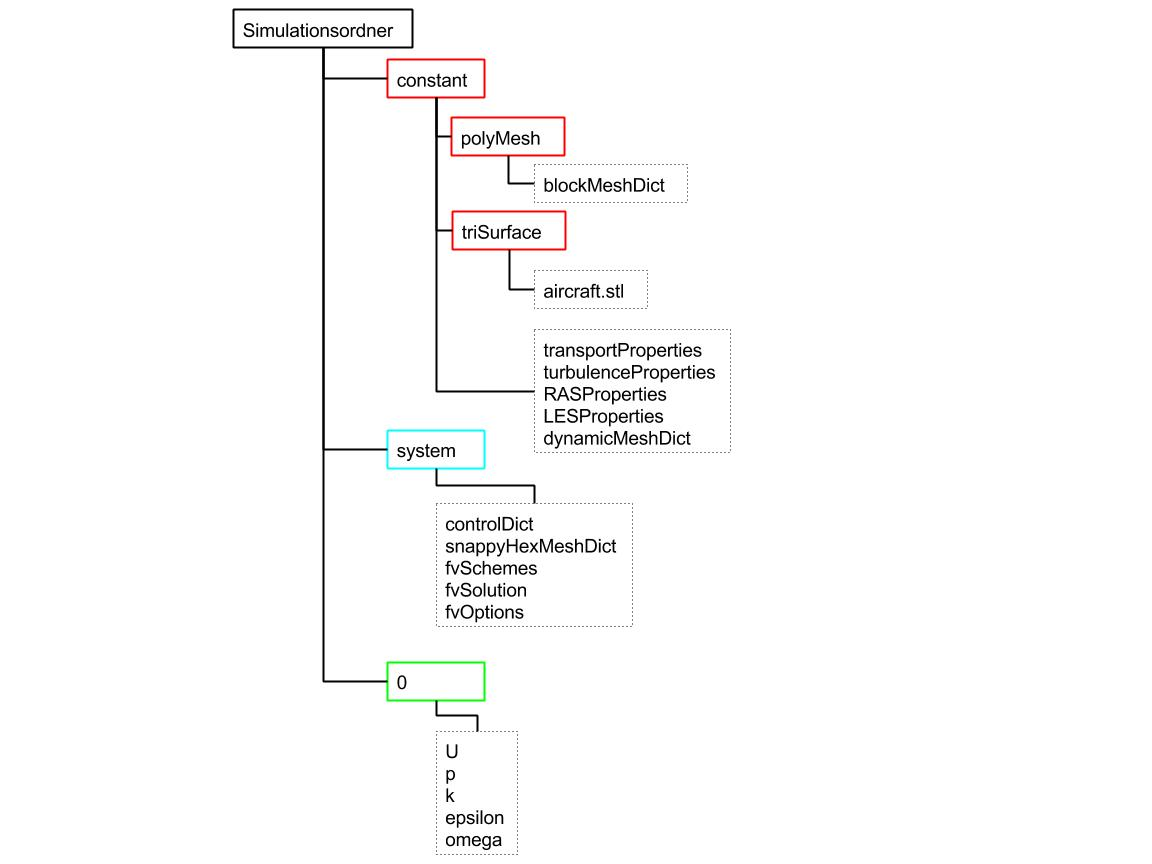
\includegraphics[width=\linewidth]{Abbildungen/Struktur}
\caption[Struktur einer OpenFOAM Simulation]{Die Ordnerstruktur innerhalb einer OpenFOAM Simulation. Der system ordner beinhaltet die Einstellungen der Lösungsprogramme, der 0 Ordner beinhaltet die Initialbedingungen und der constant Ordner das Gitter und die Randbedingungen}
\label{fig:struktur}
\end{figure}

\subsection{\texttt{constant}}
Der \textit{constant} Ordner beinhaltet im Subordner polyMesh das von numerische Gitter im OpenFOAM Format. Handelt es sich bei dem Gitter um ein mit \textit{blockMesh} generiertes blockstrukturiertes Gitter, so liegt dort auch die Datei \textit{blockMeshDict}, Siehe \autoref{lst:blockMeshDict}, innerhalb derer die Geometrie und die Randbedingungen definiert werden. Des Weiteren beinhaltet \textit{constant} unter Umständen das Unterverzeichnis \textit{triSurface}, innerhalb dessen Oberflächengitter zur Generierung komplexer Gitter mit den Gittergeneratoren \textit{snappyHexMesh}, \textit{foamyQuadMesh} und \textit{foamyHexMesh} abgelegt sind (Siehe Kapitel Gittergenerierung).

Zwangsweise vorhanden sein muss die Datei transportProperties. Diese Datei legt die kinematische Viskosität sowie die Art von Fluid (Newtonsch, Binghamsch, etc.) fest.

In den Dateien RASProperties, LESProperties und turbulenceProperties werden etwaige Turbulenzemodelle definiert. 

Eine gesonderte Rolle spielte die Datei dynamicMeshDict; Soll innerhalb der Simulation mit bewegten Gittern gearbeitet werden, so wird das Verfahren, sowie die Bewegung hier definiert.

\subsection{\texttt{system}}
Mit den Dateien innerhalb dieses Ordners wird die Simulation gesteuert.

\begin{itemize}
	
	\item[\textbf{\textit{controlDict}}] Mit dieser Datei wird die Simulation gesteuert; nachfolgend sind die wichtigsten Parameter und ihre Optionen aufgeführt.
		\subitem application : legt den zu verwendenden Gleichungslöser fest; nicht zwingend notwending, nur in Kombination mit den von OpenFOAM bereitgestellten RunFunctions benötigt.
		
		\subitem startFrom : legt fest ob die Simulation von einem festgelegten Zeitpunkt aus startet oder vom letzten verfügbaren Zeitschritt. Soll ein Zeitschritt festgelegt werden, muss als Wert 'startTime' eingetragen werden. Ansonsten 'latestTime'. 
		
		\subitem startTime : wird nur benötigt falls ein fester Startzeitpunkt festgelegt werden soll. 
		
		\subitem endTime : definiert das Ende der Simulation. 
		
		\subitem deltaT : bezeichnet die Zeitschrittweite und bei instationären Simulationen damit die Courantzahl. Bei stationären Zeitschritten ist die Zeitschrittweite überflüssig, auf 1 gesetzt zeigt sie somit die Anzahl an Iterationen an. 
		
		\subitem writeControl : steuert das Speichern. Soll der momentan gerechnete Zeitschritt noch beendet werden und danach die Simulation abgeschlossen, muss als Wert 'writeNow' eingetragen werden. Andere Optionen sind timeStep und XXX \todo{anderen Parameter raussuchen}.
		
		\subitem writeInterval : definiert die Speicherintervalle.
		
		\subitem writeFormat : definiert ob beim speichern die Daten in binärem Format oder in menschlich-lesbarem (ascii) gespeichert werden sollen. Binary reduziert den benötigten Speicherplatz auf etwa 20 \% des menschlich-lesbaren.
		
		\subitem runTimeModifiable : lässt zu ob Textdateien zur Kontrolle der Simulation geändert und damit die Simulation zur Laufzeit modifiziert werden darf.
		
		\subitem functions : Soll zur Laufzeit bereits PostProcessing betrieben werden (bspw: grafische Schnitte, Strömungsbeiwerte, etc), müssen diese hier definiert werden
	
	\item[\textbf{\textit{snappyHexMeshDict}}] Diese Datei wird als Steuerdatei für den Gittergenerator \textit{snappyHexMesh} benötigt. Details dazu finden sich im Kapitel Gittergenerierung.
		
	\item[\textbf{\textit{fvSchemes}}] Diese Datei beinhaltet die zu verwendenden Diskretisierungs und Interpolationsverfahren. Grundsätzlich gibt es in OpenFOAM viele verschiedene Verfahren. Erforderlich für das Starten einer Simulation ist zunächst, dass alle in den vorhandenen Gleichungen auftretenden Terme durch die Verfahren abgedeckt sind. \autoref{tab:terme} zeigt die Terme und ihre Bezeichnungen in OpenFOAM. Das Kapitel Diskretisierungen behandelt die vorhandenen Verfahren und ihre Effekte.
	
	\begin{table}[htb]
	  \centering
	  \begin{tabular}{m{6cm}m{3cm}} 
	  \toprule
	    	Term & Bezeichnung in OpenFOAM \\
	  \midrule
			Instationärer Term $ \frac{\partial u_{i}}{\partial t} $ & \texttt{ddtSchemes} \\
			Konvektiver Term $ u_{j} \frac{u_{i}}{x_{j}} $ & \texttt{divSchemes} \\
			(Druck)Gradient $ - \frac{ \frac{p}{\rho} + g k}{\partial x_{i}} $ & \texttt{gradSchemes} \\
			Diffusiver Term $ \nu \frac{\partial^{2} u_{i}}{\partial u_{j}^{2}} $& \texttt{laplacianSchemes} \\
			Interpolationsverfahren & \texttt{interpolationSchemes} \\
	  \bottomrule
	  
	  \end{tabular}
	  \caption[Terme und ihre Bezeichnungen in OpenFOAM]{Terme und ihre Bezeichnungen in OpenFOAM}
	  \label{tab:terme}
	\end{table} 
	
	\item[\textbf{\textit{fvSolution}}] Innerhalb dieser Datei werden die Algorithmen zur Gleichungslösung eingestellt. Des Weiteren werden Ralaxationsfaktoren und Konvergenzkriterien hier definiert. 
	
	\item[\textbf{\textit{fvOptions}}] Diese Datei beinhaltet die Beschreibung bestimmter Patches, beispielsweise zur Simulation von porösen Medien oder zur Simulation mit anderen Bezugssystemen. 
	
\end{itemize}

\subsection{\texttt{0}}
Innerhalb des '0' Ordners werden die Initialbedingungen festegelegt; alle zur Simulation benötigten Größen erhalten ihre eigene Datei, innerhalb derer die Initialwerte festgelegt werden. Für Details: Kapitel Initial und Randbedingungen. 




\newpage
\chapter{Gittergenerierung}

\section{blockMesh}
\textit{blockMesh} ist ein einfacher Gittergenerator für blockstrukturierte (Hexaeder) Gitter. \textit{blockMesh} benötigt als input die datei \textit{constant/polyMesh/blockMeshDict} in welcher die Geometrie und Gittergenerierung festgelegt werden. \autoref{fig:blockmesh} zeigt ein solches Gitter.
\\
Aufgerufen wird \textit{blockMesh} normalerweise ohne Parameter im Wurzelordner der Simulation.

\begin{figure}[htb]
  \centering
  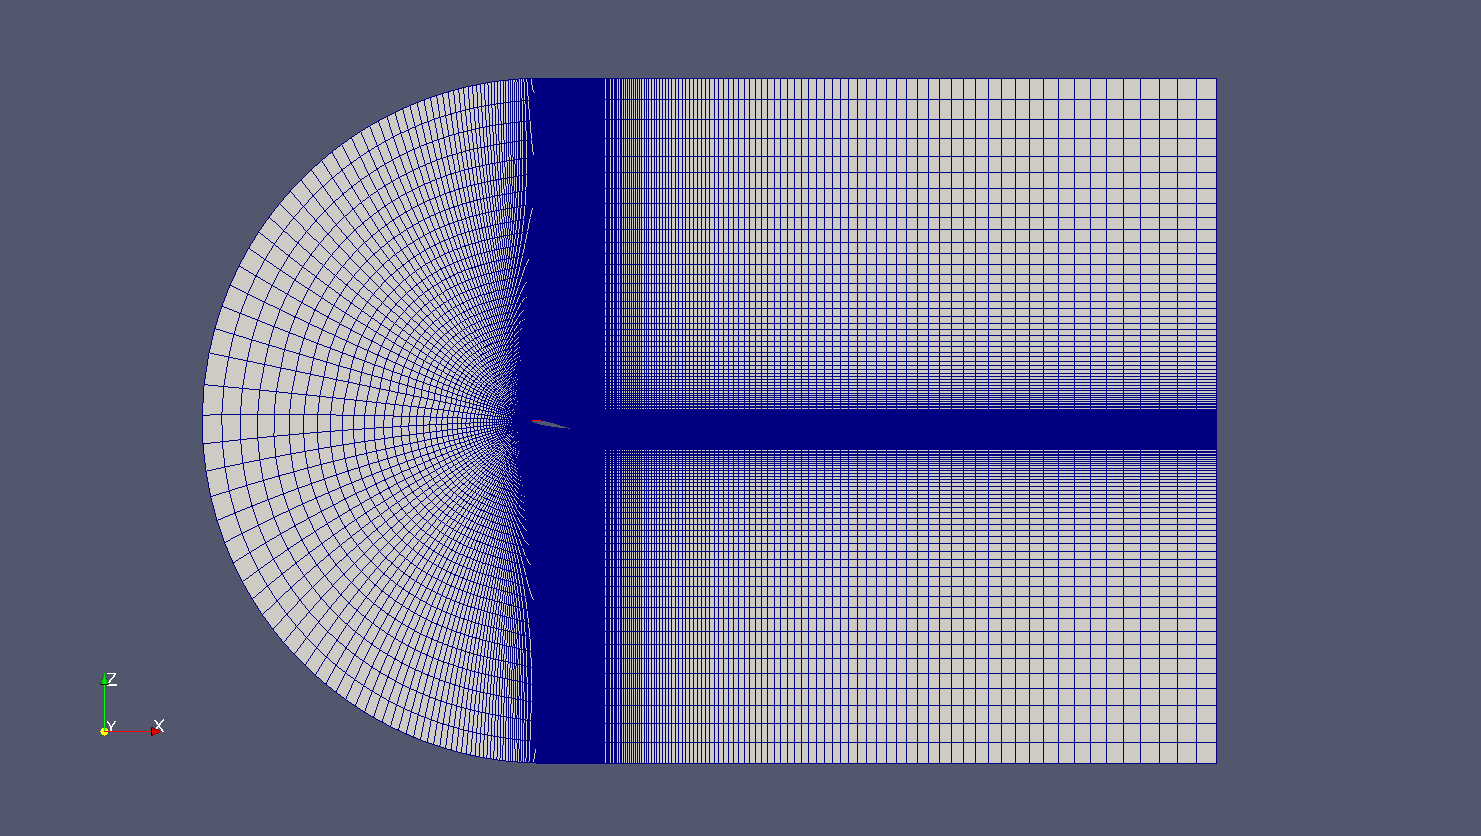
\includegraphics[width=0.95\linewidth]{Abbildungen/blockmesh} 
  \caption[blockMesh Gitter]{Ein mit \textit{blockMesh} generiertes Gitter eines NACA 0012 Flügelprofils. Deutlich zu erkennen ist das Grading im Gitter.}
  \label{fig:blockmesh}
\end{figure}

\autoref{lst:blockMeshDict} zeigt das zur Generierung des in \autoref{fig:blockmesh} genutzte \textit{blockMeshDict}.


Grundsätzlich ist die Gittergenerierung relativ einfach, einige Punkte sind jedoch zu beachten: 
\begin{itemize}
  \item scaleToMeters: Der Parameter \textit{scaleToMeters} (Zeile 18 in \autoref{lst:blockMeshDict}) \textit{blockMeshDicts} ermöglicht es die zu erstellenden Gitter automatisch zu skalieren. Dieser Parameter kann schnell zu Fehlern in den Rechnungen führen, da die Größe des Gitters nicht sofort erkennbar ist und dadurch die zu simulierenden Größen, welche von der Gitterlänge (bspw. Geschwindigkeit, kinematische Viskosität) schnell um Größenordnungen abweichen können. 
  \item boundary: Die Randbedingungen der Gitter werden bereits im \textit{blockMeshDict} festgelegt (in \autoref{lst:blockMeshDict} ab Zeile 116). Dabei ist wichtig, dass die richtig Option gewählt wird. Es stehen in OpenFOAM verschiedene Randbedingungen zur Verfügung (Siehe dazu Kapitel OpenFOAM). Ist noch nicht sicher, um welche Art Randbedingung es sich handelt, ist \textit{type patch} die beste Wahl. 
  \item Uhrzeigersinn: Sollte es beim Generieren des Gitters zu Schwierigkeiten kommen, so lohnt es sich immer die Reihenfolge der abgezählten Knoten (\textit{vertices}) zu überprüfen. Sind diese nicht in der richtigen Reihenfolge kommt es zu Verdrehungen innerhalb des Gitters.
\end{itemize}

\newpage

\section{snappyHexMesh}

\textit{snappyHexMesh} generiert aus einem blockstrukturierten Gitter (blockMesh) ein hybrides Gitter. Mit diesem Tool können bequem komplexe Geometrien in Gitter umgesetzt werden. \autoref{fig:snappy_geometry} zeigt den schematischen Aufbau. Dabei wird von der komplexen Geometrie ein Oberflächengitter (In \autoref{fig:snappy_geometry} als STL surface bezeichnet) benötigt, welches von dem blockstrukturietem Gitter umgeben ist. Das Tool unterstützt viele Oberflächengitter (u.a.: STLs). Als zusätzliche Fähigkeit können prismatische Oberflächenzelle generiert werden, welche (Druck)Gradienten besser abbilden können. Das Tool ist voll parallelisiert, diese Möglichkeit sollte auch genutzt werden, da der Speicherverbrauch hoch ist (pro 1Mio Zellen etwa 1 GB RAM)
\\
Der Aufruf von \textit{snappyHexMesh} erfolgt aus dem Wurzelordner der Simulation. Als nützliche Parameter seinen hier die folgenden aufgezählt:
\begin{itemize}
	\item \texttt{-parallel} soll \textit{snappyHexMesh} parallel genutzt werden, so ist dieser Parameter unerlässlich.
	\item \texttt{-overwrite} \textit{snappyHexMesh} schreibt alle drei Bearbeitungschritte in eigene Zeitordner; ist dies nicht gewünscht (da meist unpraktikabel), hilft dieser Parameter. Das Gitter wird in den \texttt{constant} Ordner geschrieben.
\end{itemize}
\begin{figure}
\centering
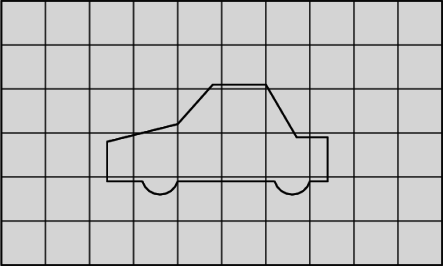
\includegraphics[width=0.7\linewidth]{Abbildungen/snappy_geometry2}
\caption[Geometriedefinition snappyHexMesh]{Geometrie innerhalb eines blockstrukturierten Gitters für die Gittergeneration mit snappyHexMesh. Das blockstrukturierte Gitter muss die Oberfläche überall dort umschließen, wo es zu einer Interaktion zwischen Fluid und Geometrie kommen soll.}
\label{fig:snappy_geometry}
\end{figure}


\textit{snappyHexMesh} wird durch eine Inputdatei (\textit{system/snappyHexMeshDict}) gesteuert. Die Gittergenerierung mit \textit{snappyHexMesh} lässt sich in drei Schritte unterteilen.
\begin{itemize}
	\item Verfeinern	(\textit{castellatedMesh})
	\item Glätten		(\textit{snap})
	\item Oberflächenzellen hinzufügen	(\textit{addLayers})
\end{itemize}
Das \textit{snappyHexMeshDict} ist diesen Schritten entsprechend gegliedert. Zunächst wird die Geomtrie festgelegt (\autoref{lst:snappyHexMeshDictGeometry}):

\begin{dict}{Geometriedefinition innerhalb von \textit{snappyHexMeshDict}}{lst:snappyHexMeshDictGeometry}[ht]
geometry
{
    oberflaeche.stl
    {
        type triSurfaceMesh;
        name oberflaeche;
    }

    verfeinerung
    {
        type searchableBox;
        min (-1.0 -0.7 0.0);
        max ( 8.0  0.7 2.5);
    }
};
\end{dict}

Dabei sind in \textit{snappyHexMesh} mehrere Typen von Geometrien erlaubt:
\begin{itemize}

	\item \texttt{closedTriSurfaceMesh}: benötigt als Input eine \underline{geschlossene} Oberflächengeometrie
	\item \texttt{distributedTriSurfaceMesh}: \todo{raus finden was das ist}
	\item \texttt{searchableBox}: generiert eine Box über die längste Diagonale fest. Inputparameter sind \textit{min(x y z)} und \textit{max(x y z)}.
	\item \texttt{searchableCylinder}: generiert einen Zylinder. Inputparameter sind \textit{min (x y z)}, \textit{max(x y z)} und \textit{radius r}.
	\item \texttt{searchableDisk} \todo{testen}
	\item \texttt{searchablePlane} \todo{testen}
	\item \texttt{searchablePlate} \todo{testen}
	\item \texttt{searchableSphere}: generiert eine Kugel. Inputparameter sind \textit{radius r} und \textit{centre (x y z)}
	\item \texttt{searchableSurfaceCollection} \todo{dafuq?}
	\item \texttt{searchableSurfaceWithGaps} \todo{dafuq?}
	\item \texttt{triSurfaceMesh}: benötigt als Input eine Oberflächengeometrie. 
	
\end{itemize}

Danach folgen die Einstellung für das Verfeinern der Zellen, dem ersten Schritt innerhalb von \textit{snappyHexMesh} (\textit{castellatedMeshControls})

\begin{dict}{\textit{castellatedMeshControls} innerhalb von \textit{snappyHexMeshDict}}{lst:snappyHexMeshDictCastellated}
castellatedMeshControls
{
	// maximal zulässige Anzahl von Zellen pro Prozessor
	// ACHTUNG: bricht Verfeinerung ab sobald Anzahl erreicht ist
    maxLocalCells 100000;

	// maximal zulässige Anzahl von Zellen über alle Prozessoren summiert
    // ACHTUNG: bricht Verfeinerung ab sobald Anzahl erreicht ist
    maxGlobalCells 2000000;

	// sollten weniger als diese Anzahl an Zellen verfeinert werden, wird abgebrochen
    minRefinementCells 10;

	// maximal zulässiges Ungleichgewicht an Zellanzahlen zwischen Prozessoren. Wird dieses Niveau überschritten, werden die Zellen neu verteilt
    maxLoadUnbalance 0.10;

	// Anzahl an Zellschichten zwischen den Verfeinerungen
    nCellsBetweenLevels 3;

	// wird das zusätzliche Tool surfaceFeatureExtract genutzt wird die davon generierte Geometrie hier eingebunden und das Verfeinerungslevel festegelegt
    features
    (
        {
            file "motorBike.eMesh";
            level 6;
        }
    );

	// die Oberflächen zu denen hin verfeinert werden soll, werden hier festgelegt. Dabei kann es sich sowohl um die vorher eingelenen Oberflächengeometrien aus dateien als auch um intern festgelegte Geomtrien, bsp searchableSphere handeln.
    refinementSurfaces
    {
        oberflaeche
        {
            level (min max);
        }
    }

	// Dieser Winkel zwischen zwei angrenzenden Zellen entscheidet darüber, ab wann das nächste Verfeinerungslevel an der Oberfläche eingesetzt werden soll. Start bei min.
    resolveFeatureAngle 45;

	// Soll ein ganzer Zellbereich innerhalb eines bestimmten Raumes auf ein bestimmtes Maß verfeinert werden, wird dies hier festgelegt
    refinementRegions
    {
        refinementBox
        {
            mode inside;
            levels ((1E15 4));
        }
    }

	// diese Koordinate entscheidet darüber welcher Teil des Gitters behalten wird; der innerhalb der Geometrie oder der ausserhalb.
    locationInMesh (3.0001 3.0001 0.43);

	\todo{was ist das?}
    allowFreeStandingZoneFaces true;
}\end{dict}

Nach dem dieser Schritt abgeschlossen ist, ist das Gitter sowohl innerhalb als auch ausserhalb der Geometrie zur Geometrie hin verfeinert (siehe \autoref{fig:snappy_refinement}). 

\begin{figure}
\centering
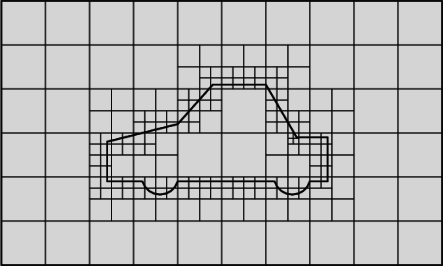
\includegraphics[width=0.7\linewidth]{Abbildungen/snappy_refinement}
\caption[Zellverfeinerung snappyHexMesh]{Die Zellverfeinerungen in der Umgebung der Oberflächengeometrie.}
\label{fig:snappy_refinement}
\end{figure}

Mit Hilfe des Parameters \texttt{locationInMesh (x y z)} wird nun entschieden welcher Teil des Gitter erhalten wird und welcher Teil entfernt wird. Dies gilt ausdrücklich nur wenn es sich bei der Geometrie um eine Wand handelt. Es ist grundsätzlich auch möglich die Verfeinerungen in beide Richtungen beizubehalten. 
\\
Nach dem Ausschneiden sieht das Gitter wie folgt aus (\autoref{fig:snappy_castellated}):

\begin{figure}
\centering
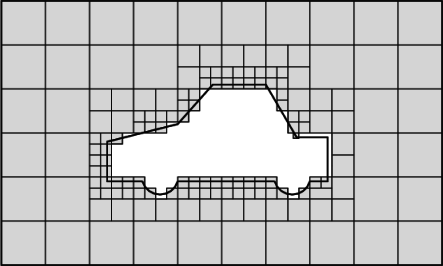
\includegraphics[width=0.7\linewidth]{Abbildungen/snappy_castellated}
\caption[Ungeglättetes, verfeinertes Gitter in snappyHexMesh]{Das ungeglättete, verfeinerte Gitter in snappyHexMesh.}
\label{fig:snappy_castellated}
\end{figure}

Auf die Einstellungen für die Verfeinerungen folgen die Einstellungen für das Glätten der Oberfläche, der zweite Schritt innerhalb von \textit{snappyHexMesh} (\textit{snapControls}, \autoref{lst:snappyHexMeshDictSnap})

\begin{dict}{\textit{snapControls} innerhalb von \textit{snappyHexMeshDict}}{lst:snappyHexMeshDictSnap}
snapControls
{
	// Dieser Parameter legt fest wie viele Iterationen (Wiederholungen) snappyHexMesh darauf verwenden darf die Oberfläche zu glätten.
    nSmoothPatch 3;

	// Dieser Faktor legt die Auflösungtoleranz fest; Die tatsächliche Toleranz entspricht der lokalen Kantenlänge multipliziert mit diesem Faktor. 
    tolerance 2.0;

	// Lösungsiterationen des Gleichungslösers, welcher die Gitterpunkte verschiebt
    nSolveIter 30;

	// Relaxationsiterationen für den Gleichungslöser	
    nRelaxIter 5;

	// Die folgenden Parameter gelten nur für den Fall das mit surfaceFeatureExtract gearbeitet wurde
    nFeatureSnapIter 10;

    implicitFeatureSnap false;

    explicitFeatureSnap true;

    multiRegionFeatureSnap false;
}
\end{dict}

Nach erfolgreicher Beendigung dieses Schrittes hat das Gitter folgende Form (\autoref{fig:snappy_smoothing}):
\begin{figure}
\centering
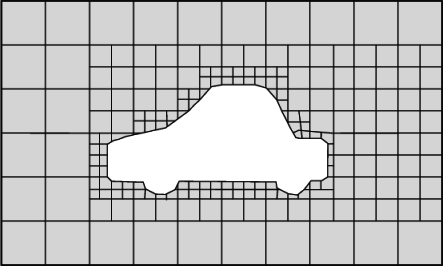
\includegraphics[width=0.7\linewidth]{Abbildungen/snappy_smoothing}
\caption[geglättetes Gitter mit snappyHexMesh]{Das an der Oberfläche geglättete Gitter.}
\label{fig:snappy_smoothing}
\end{figure}

Im letzten Schritt werden die Prismenschichten an den festgelegten Oberflächen generiert. Hierzu werden die folgenden Einstellungen benötigt (\autoref{lst:snappyHexMeshDictAddLayers}):

\begin{dict}{\textit{addLayerControls} innerhalb von \textit{snappyHexMesh}}{lst:snappyHexMeshDictAddLayers}
addLayersControls
{
    // Hier wird angegeben, ob es sich um zum Grundgitter relative Größenangaben (true) oder um absolute Größenangaben (false) handelt. 
    relativeSizes true;

    layers
    {
        geometriename    //nicht name der datei, sondern der name des patches
        {
            nSurfaceLayers 3;
        }
    }

	// relativer Wachstumsfaktor
    expansionRatio 1.0;
	
	// relative Dicke der letzen prismatischen Zellschicht zur unveränderten Grundgitterzelle
    finalLayerThickness 0.3;

	// relative Mindestdicke
    minThickness 0.1;

	// sollten bestimmte Bereich nicht mit Zellen bedeckt werden können, kann die Anzahl der nGrow Iterationen helfen Bedeckung zu erreichen.
    nGrow 0;

	// Ab welchem Winkel zwischen zwei Zellen sollen keine Zellen mehr generiert werden
    featureAngle 60;

	// finger weg \todo{dafuq tis shit?}
    slipFeatureAngle 30;

	// relaxationsiterationen
    nRelaxIter 3;

	// iterartionen zum Glätten der Flächennormalen 
    nSmoothSurfaceNormals 1;

    // Glättungsiterationen des internen Gitters
    nSmoothNormals 3;

   	// iterationen zum glätten der Zellschichtdicken
    nSmoothThickness 10;

    // Ab wann das Glätten der Dicke unterbrochen werden soll; entspricht dem Verhältnis von Zelldicke zu Fläche
    maxFaceThicknessRatio 0.5;

	// keine ahnung
    maxThicknessToMedialRatio 0.3;

	// ebenfalls keine ahnung
    minMedianAxisAngle 90;

    // bis hier her hat eh niemand gelesen
    nBufferCellsNoExtrude 0;

	// Maximale Iteration von Iterationen
    nLayerIter 50;
}
\end{dict}

\begin{figure}
\centering
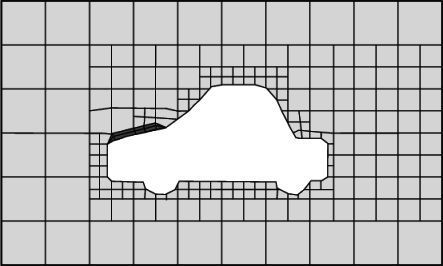
\includegraphics[width=0.7\linewidth]{Abbildungen/snappy_addlayers}
\caption[Prismenschichten snappyHexMesh]{Die Abbildung zeigt das Hinzufügen von prismatischen Zellschichten an der Oberfläche der Geometrie.}
\label{fig:snappy_addlayers}
\end{figure}


\section{proprietäre Gittergeneratoren}

Es existieren eine Reihe freiere und propritärer Gittergeneratoren, für welche OpenFOAM Konvertierungstools zur Verfügung stellt.

\begin{itemize}
	\item[liste:]
\end{itemize}

\newpage
\chapter{Diskretisierungen und Gleichungslöser}

\section{Diskretisierungsverfahren: \texttt{fvSchemes}}

% auf listing verweisen

\subsection{Zeitliche Diskretisierung: \texttt{ddtSchemes}}

\textsc{OpenFOAM} stellt folgende zeitliche Diskretisierungsverfahren zur Verfügung:

\begin{itemize}
	\item \texttt{CoEuler}
	\item \texttt{CrankNicolson}
	\item \texttt{Euler}
	\item \texttt{SLTS}
	\item \texttt{backward}
	\item \texttt{bounded}
	\item \texttt{localEuler}
	\item \texttt{steadyState}
\end{itemize} 

\subsection{Konvektiver Term: \texttt{divSchemes}}

CoBlended
Gamma
GammaV
LUST
MUSCL
MUSCLV
Minmod
MinmodV
OSPRE
OSPREV
Phi
QUICK
QUICKV
SFCD
SFCDV
SuperBee
SuperBeeV
UMIST
UMISTV
biLinearFit
blended
clippedLinear
cubic
cubicUpwindFit
downwind
filteredLinear
filteredLinear2
filteredLinear2V
filteredLinear3
filteredLinear3V
fixedBlended
limitWith
limitedCubic
limitedCubicV
limitedLinear
limitedLinearV
limiterBlended
linear
linearFit
linearPureUpwindFit
linearUpwind
linearUpwindV
localBlended
localMax
localMin
midPoint
outletStabilised
pointLinear
quadraticFit
quadraticLinearFit
quadraticLinearUpwindFit
quadraticUpwindFit
reverseLinear
skewCorrected
upwind
vanAlbada
vanAlbadaV
vanLeer
vanLeerV
weighted


\subsection{Gradienten: \texttt{gradSchemes}}

CoBlended
Gamma
Gamma01
LUST
MUSCL
MUSCL01
Minmod
OSPRE
QUICK
SFCD
SuperBee
UMIST
biLinearFit
blended
clippedLinear
cubic
cubicUpwindFit
downwind
filteredLinear
filteredLinear2
filteredLinear3
fixedBlended
harmonic
limitWith
limitedCubic
limitedCubic01
limitedGamma
limitedLimitedCubic
limitedLimitedLinear
limitedLinear
limitedLinear01
limitedMUSCL
limitedVanLeer
limiterBlended
linear
linearFit
linearPureUpwindFit
linearUpwind
localBlended
localMax
localMin
midPoint
outletStabilised
pointLinear
quadraticFit
quadraticLinearFit
quadraticLinearUpwindFit
quadraticUpwindFit
reverseLinear
skewCorrected
upwind
vanAlbada
vanLeer
vanLeer01
weighted

\subsection{Diffusiver Term: \texttt{laplacianSchemes}}

CoBlended
Gamma
Gamma01
LUST
MUSCL
MUSCL01
Minmod
OSPRE
QUICK
SFCD
SuperBee
UMIST
biLinearFit
blended
clippedLinear
cubic
cubicUpwindFit
downwind
filteredLinear
filteredLinear2
filteredLinear3
fixedBlended
harmonic
limitWith
limitedCubic
limitedCubic01
limitedGamma
limitedLimitedCubic
limitedLimitedLinear
limitedLinear
limitedLinear01
limitedMUSCL
limitedVanLeer
limiterBlended
linear
linearFit
linearPureUpwindFit
linearUpwind
localBlended
localMax
localMin
midPoint
outletStabilised
pointLinear
quadraticFit
quadraticLinearFit
quadraticLinearUpwindFit
quadraticUpwindFit
reverseLinear
skewCorrected
upwind
vanAlbada
vanLeer
vanLeer01
weighted


\subsection{Interpolation: \texttt{interpolationSchemes}}

CoBlended
Gamma
Gamma01
LUST
MUSCL
MUSCL01
Minmod
OSPRE
QUICK
SFCD
SuperBee
UMIST
biLinearFit
blended
clippedLinear
cubic
cubicUpwindFit
downwind
filteredLinear
filteredLinear2
filteredLinear3
fixedBlended
harmonic
limitWith
limitedCubic
limitedCubic01
limitedGamma
limitedLimitedCubic
limitedLimitedLinear
limitedLinear
limitedLinear01
limitedMUSCL
limitedVanLeer
limiterBlended
linear
linearFit
linearPureUpwindFit
linearUpwind
localBlended
localMax
localMin
midPoint
outletStabilised
pointLinear
quadraticFit
quadraticLinearFit
quadraticLinearUpwindFit
quadraticUpwindFit
reverseLinear
skewCorrected
upwind
vanAlbada
vanLeer
vanLeer01
weighted


\section{Gleichungslöser: \texttt{fvSolution}}

\subsection{Symmetrische Matrizen}

\paragraph{Gleichungslöser}
GAMG
ICCG
PCG
smoothSolver

\paragraph{Gläätungsalgorithmen}

DIC
DICGaussSeidel
FDIC
GaussSeidel
nonBlockingGaussSeidel
symGaussSeidel




% auf listing verweisen
		

\newpage
\chapter{Inital und Randbedingungen}

In diesem Bereich passieren die meisten Fehler; aus diesem Grund sollte hier mit besonderer Vorsicht und Konzentration gearbeitet werden.

Die Initial und Randbedingungen verteilen sich auf zwei Ordner: \textit{0} und \textit{constant}

Es müssen an allen Rändern Randbedingungen definiert werden.

Grundsätzlich unterscheidet \textsc{OpenFOAM} zwischen verschiedenen Patch-typen: \textit{base type}, \textit{primitve type} und \textit{derived type}. Dabei bedeutet \textit{base type} einfachste geometrische Definitionen. Es gibt nut zwei verschiedene Arten: \texttt{patch} und \texttt{wall}.

Aus dem \textit{base type} ergeben sich die \textit{primitive types} für die Größe $ \Phi $ (siehe \autoref{tab:primitive}): 
	
	\begin{table}[htb]
	  \centering
	  \begin{tabular}{m{2.5cm}m{6cm}m{3cm}} 
	  \toprule
	    	Typ & Beschreibung & Festzulegende Werte \\
	  \midrule
			\texttt{fixedValue} & Wert für $ \Phi $ muss festgelegt werden & \texttt{value} \\
			\texttt{fixedGradient} & Der Gradient für $ \Phi $ muss festgelegt werden & \texttt{gradient} \\
			\texttt{zeroGradient} & Der Gradient von $ \Phi $ ist null & - \\
			\texttt{calculated} & Die Werte für $ \Phi $ werden durch andere Größen bestimmt & - \\
			\texttt{mixed} & Mischt \texttt{fixedValue} und \texttt{fixedGradient} abhängig vom Wert in 	\texttt{valueFraction} & \texttt{refValue, refGradient, valueFraction, value} \\
			\texttt{directionMixed} & wie \texttt{valueFraction}, jedoch mit \texttt{valueFraction} als Tensor, sodass sich verschiedene Mischlevel in Normal- und Tangentialrichtung ergeben. & \texttt{refValue, refGradient, valueFraction, value} \\
	  \bottomrule
	  
	  \end{tabular}
	  \caption[Terme und ihre Bezeichnungen in OpenFOAM]{Terme und ihre Bezeichnungen in OpenFOAM}
	  \label{tab:primitive}
	\end{table} 

Aus der Kombination dieser Typen lassen sich die sog. \textit{derived types} herleiten. Da es insgesamt 67 dieser Randbedingungen gibt, werden nachfolgend nur die wichtigsten aufgeführt. 


SRFFreestreamVelocity
SRFVelocity
activeBaffleVelocity
activePressureForceBaffleVelocity
advective
atmBoundaryLayerInletVelocity
calculated
codedFixedValue
codedMixed
cyclic
cyclicACMI
cyclicAMI
cyclicSlip
cylindricalInletVelocity
directionMixed
empty
externalCoupled
fixedGradient
fixedInternalValue
fixedJump
fixedJumpAMI
fixedMean
fixedNormalInletOutletVelocity
fixedNormalSlip
fixedValue
flowRateInletVelocity
fluxCorrectedVelocity
freestream
inletOutlet
interstitialInletVelocity
kqRWallFunction
mapped
mappedField
mappedFixedInternalValue
mappedFixedPushedInternalValue
mappedFlowRate
mappedVelocityFlux
mixed
movingWallVelocity
nonuniformTransformCyclic
oscillatingFixedValue
outletInlet
outletMappedUniformInlet
outletPhaseMeanVelocity
partialSlip
pressureDirectedInletOutletVelocity
pressureDirectedInletVelocity
pressureInletOutletParSlipVelocity
pressureInletOutletVelocity
pressureInletUniformVelocity
pressureInletVelocity
pressureNormalInletOutletVelocity
processor
processorCyclic
rotatingPressureInletOutletVelocity
rotatingWallVelocity
sliced
slip
supersonicFreestream
surfaceNormalFixedValue
swirlFlowRateInletVelocity
symmetry
symmetryPlane
timeVaryingMappedFixedValue
translatingWallVelocity
turbulentInlet
uniformFixedGradient
uniformFixedValue
uniformInletOutlet
uniformJump
uniformJumpAMI
variableHeightFlowRateInletVelocity
waveTransmissive
wedge
zeroGradient

\newpage
\chapter{Pre-Processing}

\newpage
\chapter{Stationäre Rechnungen}

\section{\texttt{SIMPLE}-Algorithmus: \textsc{simpleFoam}}

\texttt{SIMPLE} steht für \textit{Semi-Implicit Method for Pressure Linked Equations}. Dieses numerische Verfahren ist ein iterativer Algorithmus zum lösen der stationären Navier-Stokes-Gleichungen.

Die iterativen Schritte sind wie folgt:

\begin{enumerate}
\item Die Randbedingungen setzen
\item Die Gradienten von Druck und Geschwindigkeit berechnen
\item Die diskretisierte Impulsgleichung lösen um das innere Geschwindigkeitsfeld zu berechnen
\item Berechne den (unkorrigierten) Masseflux an den Zellflächen
\item Löse die Druckkorrekturgleichung für alle Zellen
\item Korrigiere das Druckfeld: $ p^{k+1} = p^{k} + f_{relax} \cdot p´ $, mit $ f_{relax} $ = Relaxationsfaktor für $ p $
\item Korrigiere den Druck an den Randbedingungen
\item Korrigiere den Massenfluss an den Zellflächen
\item Korrigiere die Geschwindigkeiten in den Zellen
\item Berechne die Dichte neu (Änderungen sind durch Druckänderungen möglich)
\end{enumerate}

\newpage
\chapter{Instationäre Rechnugen}

\section{\texttt{PIMPLE}-Algorithmus: \textsc{pimpleFoam}}

\texttt{PIMPLE} steht für \textit{merged PIso siMPLE}.

\section{\texttt{PISO}-Algorithmus: \textsc{pisoFoam}}

\section{\texttt{ICO}-Algorithmus: \textsc{icoFoam}}

\newpage
\chapter{Bewegte Gitter}

OpenFOAM bietet vielf�ltige M�glichkeiten Bewegungen in den Simulationen abzubilden. Im folgenden Kapitel sollen die wichtigsten Methoden kurz vorgestellt und erkl�rt werden. 
\\
Zun�chst muss unterschieden werden, ob es sich bei der zu simulierenden Str�mung um eine quasistation�re Str�mung handelt, oder um eine echt instation�re. 

Zun�chst gilt es den Typ von bewegtem Gitter festzulegen. Dies geschieht �ber die Datei \textit{contant/dynamicMeshDict}.
Verf�gbare Gittertypen sind:

\begin{wraptable}{l}{3.5cm}
	\centering
	\caption{Dynamische Gittertypen}
	\small
	\begin{tabularx}{3cm}{X}
		\toprule
		Name \\
		\midrule
		dynamicInkJetFvMesh \\
		dynamicMotionSolverFvMesh \\ 
		dynamicRefineFvMesh \\
		movingConeTopoFvMesh \\
		multiSolidBodyMotionFvMesh \\
		rawTopoChangerFvMesh \\
		solidBodyMotionFvMesh \\
		staticFvMesh \\
		\bottomrule
	\end{tabularx}
	\label{tab:dynamicFvMesh}
\end{wraptable}

\newpage


\section{MRF}

F�r den Fall einer Quasistation�ren Bewegung, bspw. die Rotation einer gleichbleibenden Mixergeometrie oder Turbine bietet OpenFOAM die M�glichkeit mit sog. MRF-Solvern zu rechnen. MRF steht f�r \textit{Multi-Reference-Frame} und bedeutet, dass an Stelle eines echten bewegten Gitters in einem rotierenden Bezugssystem gerechnet wird. Dies birgt mehrere Vorteile, als auch Nachteile. Die Navier-Stokes-Gleichung verkompliziert sich durch die zus�tzlichen Terme, welche durch das Rotierende Koordinatensystem in die Gleichung einflie�en:

\begin{equation}
\label{eq:ns_rot}
	\frac{Du}{Dt} = - \frac{1}{\rho} \cdot \nabla p - 2(\Omega \times u) - (\Omega \times r) + \nu \nabla^{2} u - g k
\end{equation}

Gleichung \ref{eq:ns_rot} zeigt die Navier-Stokes Gleichung f�r ein rotierendes Bezugssystem. 
\\
Die Vorteile eines solchen Bezugssystems sind, dass keine Bewegungsgleichungen f�r die Gitterpunkte gel�st werden m�ssen. Des Weiteren ist auch keine r�umliche Interpolation der simulierten Gr��en vom alten Gitter zum neuen Gitter n�tig. Dadurch lassen sich sowohl potentielle Fehler, als auch Rechenzeit verringern. 
In der Standarddistribution (momentan: OpenFOAM 2.3.x) ist die Unterst�tzung f�r MRF grunds�tzlich enthalten, unter Anderem in \textit{simpleFoam} und \textit{pimpleFoam}.
\\
Definiert wird die Rotation durch einen Eintrag in der Datei system/fvOptions, in der eine MRF-Option definiert wird. \autoref{lst:fvOptions} listet einen Beispieleintrag aus der Datei fvOptions. Der Code ist aus einem der zu OpenFOAM geh�renden Tutorials entnommen.

\newpage

\section{AMI}

\textit{AMI} steht f�r \textit{Arbitrary Mesh Interface}, was so viel wie beliebige-Gitter-Schnittstelle bedeutet. Im Grunde genommen wird die Rechendom�ne $ \Omega $ in mehrere Bereiche Unterteilt. An den Schnittstellen dieser Bereich werden die Simulationsgr��en interpoliert. Dadurch ist eine gleitende Bewegung der Gitter zueinander m�glich, welche die Simulation von Bewegungen mit 6 Freiheitsgraden erm�glicht.
\todo{bild eines AMI-Gitters einf�gen}
\\
Um Simulationen mit dieser Technik durchzuf�hren sind mehrere Schritte n�tig. 

\newpage

\section{RBF}

\clearpage
\newpage

\section{dynamicTopoFvMesh}

Diese Bibliothek erm�glicht CFD-Simulationen mit den h�chsten Freiheitsgraden. Dies wurd durch eine dynamische Gittergenerierung zur Laufzeit der Simulationen gew�hrleistet. 
Der Code ist experimentell und die Simulationen schwer zu kontrollieren. 

Simulationen mit dieser numerischen Technik basieren auf einer Kombination aus der Gitterbibliothek \textit{Mesquite} und der eigentlichen Bibliothek \textit{dynamicTopoFvMesh}.

\textbf{Momentan ist noch ein Programmierfehler vorhanden, der das saubere durchf�hren einer dynamischen simulation verhindert, wenn der parameter \texttt{allowTableResize} auf \texttt{yes} gesetzt ist. }

\subsection{Mesquite}

Diese Bibliothek erm�glicht das Gl�tten eines numerischen Gitters. Dazu wird eine skalare Qualit�tsgr��e, welche zu jedem Zeitschritt f�r jede einzelne Gitterzelle berechnet wird genutzt. Im Nachfolgenden sind diese aufgef�hrt.

\begin{wraptable}{r}{8.5cm}
	\centering
	\caption{Qualit�tsmerkmale f�r \textit{Mesquite}}
	\small
	\begin{tabularx}{8cm}{p{4cm} p{4cm}}
		\toprule
		Name & Formel \\
		\midrule
		\textit{UntangleBeta} & \\
		\textit{AspectRatioGamma} & \\
		\textit{InverseMeanRatio} & \\
		\textit{EdgeLengthQuality} & \\
		\textit{LocalSize} & \\
		\textit{VertexConditionNumber}  & \\
		\textit{ConditionNumber}  & \\
		\textit{MeanRatio}  & \\
		\textit{EdgeLength} & \\
		\bottomrule
	\end{tabularx}
	\label{tab:qualit�t}
\end{wraptable}

\begin{wraptable}{r}{3.5cm}
	\centering
	\caption{Optimierungsalgorithmen}
	\small
	\begin{tabularx}{3cm}{X}
		\toprule
		Name \\
		\midrule
		\textit{SteepestDescent} \\
		\textit{TrustRegion} \\
		\textit{NonSmoothDescent} \\
		\textit{ConjugateGradient} \\
		\textit{SmartLaplacian} \\
		\textit{QuasiNewton} \\
		\textit{FeasibleNewton} \\
		\textit{Laplacian} \\
		\textit{Randomize} \\	
		\bottomrule
	\end{tabularx}
	\label{tab:optimierung}
\end{wraptable}

\begin{table}
	\centering
	\caption{Optimierungsalgorithmen}
	\small
	\begin{tabularx}{10cm}{m{3cm} X}
		\toprule
		Name & \\
		\midrule
		angularOscillatingDisplacement & \\
		angularOscillatingVelocity & \\
		calculated & \\
		cyclic & \\
		empty & \\
		fixedValue & \\
		generic	 & \\
		global & \\
		mixed & \\
		oscillatingDisplacement & \\
		oscillatingFixedValue & \\
		oscillatingVelocity & \\
		processor & \\
		slip & \\
		surfaceDisplacement & \\
		surfaceSlipDisplacement & \\
		symmetryPlane & \\
		timeVaryingUniformFixedValue & \\
		uniformFixedValue & \\
		value & \\
		wedge & \\
		zeroGradient  & \\
		\bottomrule
	\end{tabularx}
	\label{tab:patches_bewegung}
\end{table}

\newpage

\section{\textit{sixDoFRigidBodyMotionSolver}}



\begin{table}
	\centering
	\caption{Constraints}
	\small
	\begin{tabularx}{\linewidth}{m{2cm} X}
		\toprule
		Name & Beschreibung\\
		\midrule
		axis & Nur translative Bewegung entlang einer Achse; keine Rotation, au�er um diese Achse. Einziger ben�tigter Parameter ist die Ausrichtung der Achse \texttt{axis (x y z)}\\
		line & Erlaubt translative Bewegungen nur in Richtung der festgelegten Linie. Rotation ist ebenfalls erlaubt. Ben�tigte Parameter sind: \texttt{CentreOfRotation (x y z)} und \texttt{orientation (x y z)}\\
		orientation & \\
		plane & \\
		point & Setzt eine translative Begrenzung mit einem Punkt. Schl�sselwort ist \texttt{centreOfRotation (x y z)}. Wird dies nicht gesetzt und es werden keine anderen constraints gesetzt, wird automatisch der Masseschwerpunkt als punktrestraint gesetzt. \\
		\bottomrule
	\end{tabularx}
	\label{tab:constraintsSixDoF}
\end{table}


\begin{table}
	\centering
	\caption{Restraints}
	\small
	\begin{tabularx}{10cm}{m{3cm} X}
		\toprule
		Name & Beschreibung\\
		\midrule
		linearAxialAngularSpring & \\
		linearDamper & \\
		linearSpring & \\
		sphericalAngularDamper & \\
		sphericalAngularSpring & \\ 
		tabulatedAxialAngularSpring & \\
		\bottomrule
	\end{tabularx}
	\label{tab:restraintsSixDoF}
\end{table}

\chapter{Mehrphasenrechnungen}

\newpage
\chapter{Wärme}

\newpage
\chapter{Post-Processing}
\begin{itemize}
	\item execFlowFunctionObject
	\item vorticity
	\item yPlusRAS
	\item yPlusLES
	\item wallShearStress
	\item Q
	\item Lambda
\end{itemize}
\newpage
\chapter{Paraview}

\newpage

\chapter{Nachschlagewerke und Literatur}

\newpage

\clearpage
\pagenumbering{Roman}    %% römische (große) Seitenzahlen nach dem Hauptteil


%%---------------------------------------------------------
%% Anhang, falls erforderlich
%%---------------------------------------------------------
\appendix                %% appendix ist keine Umgebung!

%% Ab hier das Wort "Anhang" dem Kolumnentitel voranstellen
\renewcommand*{\chaptermarkformat}{\chapapp~\thechapter\autodot\enskip}
%% eine Seite mit dem Wort Anhang ausgeben (wie Kapitelanfangsseite ohne Kopfzeile)
\addchap{Anhang}       
\chapter{\texttt{constant}}

\begin{dict}{Datei \textit{constant/polyMesh/blockMesh}}{lst:blockMeshDict}

/*--------------------------------*- C++ -*----------------------------------*\ 
| =========                 |                                                 | 
| \\      /  F ield         | OpenFOAM: The Open Source CFD Toolbox           | 
|  \\    /   O peration     | Version:  2.1.0                                 | 
|   \\  /    A nd           | Web:      www.OpenFOAM.com                      | 
|    \\/     M anipulation  |                                                 | 
\*---------------------------------------------------------------------------*/ 
FoamFile                                                                        
{                                                                               
    version     2.0;                                                            
    format      ascii;                                                          
    class       dictionary;                                                     
    object      blockMeshDict;                                                  
}                                                                               
// * * * * * * * * * * * * * * * * * * * * * * * * * * * * * * * * * * * * * // 

// globale Skalierungsgröße; gilt für das gesamte Gitter
convertToMeters 1.000000; 

// Die Eckpunkte des Gitters. Im Falle dieser Geometrie die äußeren Kanten, sowie die Kanten des NACA 0012 profils. Zu beachten ist dabei, dass der erste Knoten innerhalb von OpenFOAM als Knoten 0, anstelle von Knoten 1 angesprochen wird
vertices 
( 
    (-7.530630 0.050000 1.581494)		// Knoten 0
...
    (16.000000 -0.050000 -8.000000)		//Knoten 23
); 

// Das gitter besteht insgesamt aus 6 Blöcken, welche im nachfolgenden Eintrag definiert werden. Wichtig zu beachten ist die Reihenfolge der angegebenen Kantenpunkte (vertices). Grundsätzlich ist egal in welcher Drehrichtung die Punkte angegeben werden, so lange die Drehrichtung beibehalten wird.
blocks 
( 
    hex (4 5 1 0 16 17 13 12)     (74 100 1) edgeGrading (1 0.020000 0.020000 1 500.000000 500.000000 500.000000 500.000000 1 1 1 1) 
...
    hex (19 20 23 22 7 8 11 10)   (150 100 1) simpleGrading (100.000000 500.000000 1) 
); 

// An dieser Stelle werden die Kanten des Gitters definiert. OpenFOAM stellt dafür verschiedene Verfahren zur Verfügung, unter anderem gerade Kanten (edges), Splines (spline) und Kreisbögen (arc)
edges 
( 
// Splineinterpolation entlang der angegebenen Koordinaten von Knoten 4 zu Knoten 5
    spline 4 5 
        ( 
            (0.000159 0.050000 0.000682) 
... 
            (0.301576 0.050000 -0.002021) 
        ) 
    
...
// zur Übersicht wurden die restlichen Spline-Einträge gelöscht
...        
// Kreisbogen von Knoten 0 zu Knoten 1 mit dem Verbindungspunkt in den Klammern
    arc 0 1 (-5.351755 0.050000 5.656854) 
...
    arc 12 21 (-5.351755 -0.050000 -5.656854) 
); 

// die Randbedingungen
boundary 
( 
    inlet 
    { 
        type patch; 
        faces 
        ( 
            (1 0 12 13) 
            (0 9 21 12) 
        ); 
    } 

    outlet 
    { 
        type patch; 
        faces 
        ( 
            (11 8 20 23) 
            (8 3 15 20) 
        ); 
    } 

    topAndBottom 
    { 
        type patch; 
        faces 
        ( 
            (3 2 14 15) 
            (2 1 13 14) 
            (9 10 22 21) 
            (10 11 23 22) 
        ); 
    } 

    airfoil 
    { 
        type wall; 
        faces 
        ( 
            (5 4 16 17) 
            (7 5 17 19) 
            (4 6 18 16) 
            (6 7 19 18) 
        ); 
    } 
); 
 
mergePatchPairs 
( 
); 
 
// ************************************************************************* // 


\end{dict}

\newpage
\chapter{\texttt{system}}

\begin{dict}{Datei \textit{system/fvOptions}}{lst:fvOptions}
/*--------------------------------*- C++ -*----------------------------------*\
| =========                 |                                                 |
| \\      /  F ield         | OpenFOAM: The Open Source CFD Toolbox           |
|  \\    /   O peration     | Version:  2.3.0                                 |
|   \\  /    A nd           | Web:      www.OpenFOAM.org                      |
|    \\/     M anipulation  |                                                 |
\*---------------------------------------------------------------------------*/
FoamFile
{
    version     2.0;
    format      ascii;
    class       dictionary;
    location    "system";
    object      fvOptions;
}
// * * * * * * * * * * * * * * * * * * * * * * * * * * * * * * * * * * * * * //

MRF1
{
    type            MRFSource;
    active          true;
    selectionMode   cellZone;
    cellZone        rotor;

    MRFSourceCoeffs
    {
        origin      (0 0 0);
        axis        (0 0 1);
        omega       104.72;
    }
}


// ************************************************************************* //
\end{dict}

\newpage

\begin{dict}{Datei \textit{system/fvSchemes}}{lst:fvSchemes}
/*--------------------------------*- C++ -*----------------------------------*\
| =========                 |                                                 |
| \\      /  F ield         | OpenFOAM: The Open Source CFD Toolbox           |
|  \\    /   O peration     | Version:  2.3.0                                 |
|   \\  /    A nd           | Web:      www.OpenFOAM.org                      |
|    \\/     M anipulation  |                                                 |
\*---------------------------------------------------------------------------*/
FoamFile
{
    version     2.0;
    format      ascii;
    class       dictionary;
    object      fvSchemes;
}
// * * * * * * * * * * * * * * * * * * * * * * * * * * * * * * * * * * * * * //

ddtSchemes
{
    default         steadyState;
}

gradSchemes
{
    default         Gauss linear;
    grad(U)         cellLimited Gauss linear 1;
}

divSchemes
{
    default         none;
    div(phi,U)      bounded Gauss linearUpwindV grad(U);
    div(phi,k)      bounded Gauss upwind;
    div(phi,omega)  bounded Gauss upwind;
    div((nuEff*dev(T(grad(U))))) Gauss linear;
}

laplacianSchemes
{
    default         Gauss linear corrected;
}

interpolationSchemes
{
    default         linear;
}

snGradSchemes
{
    default         corrected;
}

fluxRequired
{
    default         no;
    p;
}
\end{dict}

\newpage

\begin{dict}{Datei \textit{system/fvSolution}}{lst:fvSolution}
/*--------------------------------*- C++ -*----------------------------------*\
| =========                 |                                                 |
| \\      /  F ield         | OpenFOAM: The Open Source CFD Toolbox           |
|  \\    /   O peration     | Version:  2.3.0                                 |
|   \\  /    A nd           | Web:      www.OpenFOAM.org                      |
|    \\/     M anipulation  |                                                 |
\*---------------------------------------------------------------------------*/
FoamFile
{
    version     2.0;
    format      ascii;
    class       dictionary;
    object      fvSolution;
}
// * * * * * * * * * * * * * * * * * * * * * * * * * * * * * * * * * * * * * //

solvers
{
    p
    {
        solver           GAMG;
        tolerance        1e-7;
        relTol           0.01;
        smoother         GaussSeidel;
        nPreSweeps       0;
        nPostSweeps      2;
        cacheAgglomeration on;
        agglomerator     faceAreaPair;
        nCellsInCoarsestLevel 10;
        mergeLevels      1;
    }

    U
    {
        solver           smoothSolver;
        smoother         GaussSeidel;
        tolerance        1e-8;
        relTol           0.1;
        nSweeps          1;
    }

    k
    {
        solver           smoothSolver;
        smoother         GaussSeidel;
        tolerance        1e-8;
        relTol           0.1;
        nSweeps          1;
    }

    omega
    {
        solver           smoothSolver;
        smoother         GaussSeidel;
        tolerance        1e-8;
        relTol           0.1;
        nSweeps          1;
    }
}

SIMPLE
{
    nNonOrthogonalCorrectors 0;
}

potentialFlow
{
    nNonOrthogonalCorrectors 10;
}

relaxationFactors
{
    fields
    {
        p               0.3;
    }
    equations
    {
        U               0.7;
        k               0.7;
        omega           0.7;
    }
}

cache
{
    grad(U);
}
\end{dict}

\newpage

\begin{dict}{Datei \textit{system/controlDict}}{lst:controlDict}
/*--------------------------------*- C++ -*----------------------------------*\
| =========                 |                                                 |
| \\      /  F ield         | OpenFOAM: The Open Source CFD Toolbox           |
|  \\    /   O peration     | Version:  2.3.0                                 |
|   \\  /    A nd           | Web:      www.OpenFOAM.org                      |
|    \\/     M anipulation  |                                                 |
\*---------------------------------------------------------------------------*/
FoamFile
{
    version     2.0;
    format      ascii;
    class       dictionary;
    object      controlDict;
}
// * * * * * * * * * * * * * * * * * * * * * * * * * * * * * * * * * * * * * //

libs
(
    "libOpenFOAM.so"
    "libincompressibleTurbulenceModel.so"
    "libincompressibleRASModels.so"
);

application     simpleFoam;

startFrom       latestTime;

startTime       0;

stopAt          endTime;

endTime         500;

deltaT          1;

writeControl    timeStep;

writeInterval   100;

purgeWrite      0;


//- Uncomment to have regular (every 2 hours of run time) restart files
//secondaryWriteControl    cpuTime; // runtime
//secondaryWriteInterval   7200;    // seconds
//secondaryPurgeWrite      1;       // keep all but last dump


writeFormat     binary;

writePrecision  6;

writeCompression uncompressed;

timeFormat      general;

timePrecision   6;

runTimeModifiable true;

functions
{
    #include "readFields"
    #include "streamLines"
    #include "wallBoundedStreamLines"
    #include "cuttingPlane"
    #include "forceCoeffs"
}
\end{dict}

\newpage
\chapter{\texttt{0}}

\begin{dict}{Datei \textit{0/U}}{lst:U}
/*--------------------------------*- C++ -*----------------------------------*\
| =========                 |                                                 |
| \\      /  F ield         | OpenFOAM: The Open Source CFD Toolbox           |
|  \\    /   O peration     | Version:  2.3.0                                 |
|   \\  /    A nd           | Web:      www.OpenFOAM.org                      |
|    \\/     M anipulation  |                                                 |
\*---------------------------------------------------------------------------*/
FoamFile
{
    version     2.0;
    format      ascii;
    class       volVectorField;
    object      U;
}
// * * * * * * * * * * * * * * * * * * * * * * * * * * * * * * * * * * * * * //

dimensions      [0 1 -1 0 0 0 0];

internalField   uniform (0 0 0);

boundaryField
{
    movingWall
    {
        type            fixedValue;
        value           uniform (1 0 0);
    }

    fixedWalls
    {
        type            fixedValue;
        value           uniform (0 0 0);
    }

    frontAndBack
    {
        type            empty;
    }
}

// ************************************************************************* //
\end{dict}

\newpage

\begin{dict}{Datei \textit{0/p}}{lst:p}
/*--------------------------------*- C++ -*----------------------------------*\
| =========                 |                                                 |
| \\      /  F ield         | OpenFOAM: The Open Source CFD Toolbox           |
|  \\    /   O peration     | Version:  2.3.0                                 |
|   \\  /    A nd           | Web:      www.OpenFOAM.org                      |
|    \\/     M anipulation  |                                                 |
\*---------------------------------------------------------------------------*/
FoamFile
{
    version     2.0;
    format      ascii;
    class       volScalarField;
    object      p;
}
// * * * * * * * * * * * * * * * * * * * * * * * * * * * * * * * * * * * * * //

dimensions      [0 2 -2 0 0 0 0];

internalField   uniform 0;

boundaryField
{
    movingWall
    {
        type            zeroGradient;
    }

    fixedWalls
    {
        type            zeroGradient;
    }

    frontAndBack
    {
        type            empty;
    }
}

// ************************************************************************* //
\end{dict}

\newpage
\chapter{Formeln zu \textit{RANS-Randbedingungen}}

Formelsammlung zum abschätzen der Initalwerte für RANS-basierte Tubulenzmodelle.
Folgende Variablen haben feste Werte:

\begin{table}
  \centering
  \caption{Feste Variablen}
  \begin{tabular}{m{4cm}m{8cm}}
    \toprule
    	Variable & Wert oder Formel \\
    \midrule
    	 $ T_{u} = \frac{u'}{U} = 0.001 .. 0.1 $ & Turbulenzintesität \\
		 $ C_{\mu} = 0.09 $ & Standardvariable in vielen RANS-Modellen \\
		 $ L $ & Turbulente Längenskala \\
		 $ u' $ & Turbulente Schwankungsgeschwindigkeit	\\	 
    \bottomrule
  \end{tabular}
\end{table}

\begin{table}
  \centering
  \caption{Empirische Formeln zur Abschätzung der turbulenten Viskosität \textit{ $ \tilde{ \nu } $ } }
  \begin{tabular}{m{4cm}m{8cm}}
    \toprule
    	Formel & Anmerkung \\
    \midrule
    	 $ \tilde{\nu} = 1.2247 \cdot ( U \cdot I \cdot L ) $ & Freie Umströmung \\
    \bottomrule
  \end{tabular}
\end{table}

\begin{table}
  \centering
  \caption{Empirische Formeln zur Abschätzung der turbulenten kinetischen Energie \textit{k}}
  \begin{tabular}{m{4cm}m{8cm}}
    \toprule
    	Formel & Anmerkung \\
    \midrule
    	 $ k = 1.5 \cdot (T_{u} \cdot U_{in})^{2} $ & Freie Umströmung \\
		 $ k = T_{u}^{2} \cdot \bar{U_{in}}^{2}$ & Abgewandelte Form \\		 
    \bottomrule
  \end{tabular}
\end{table}

\begin{table}
  \centering
  \caption{Empirische Formeln zur Abschätzung der Dissipationsrate \textit{$ \varepsilon $}}
  \begin{tabular}{m{4cm}m{8cm}}
    \toprule
    	Formel & Anmerkung \\
    \midrule
    	 $ \varepsilon = \frac{ C_{\nu} \cdot k^{1.5}}{0.03 \cdot L} $ & Freie Anströmung \\
		 $ \varepsilon = \frac{ C_{\mu}^{0.75} \cdot k^{1.5}}{0.03 \cdot L} $ & Abgewandelte Form \\		 
    \bottomrule
  \end{tabular}
\end{table}

\begin{table}
  \centering
  \caption{Empirische Formeln zur Abschätzung der spezifischen Dissipationsrate \textit{$ \omega $}}
  \begin{tabular}{m{4cm}m{8cm}}
    \toprule
    	Formel & Anmerkung \\
    \midrule
    	 $ \omega = \frac{ \sqrt{k} }{ L } $ & mit L = turbulente Längenskale \\
		 $ \omega = \frac{ \varepsilon }{ k } $ & Standard \\		 
    \bottomrule
  \end{tabular}
\end{table}

\newpage
\chapter{Checkliste zu \textit{snappyHexMesh}}

Diese Checkliste orientiert sich an der allgemeinen Struktur der \textit{snappyHexMesh}-Kontrolldatei \textit{snappyHexMeshDict}.
\\
\\
\begin{Form}

\Square{} Prismatische Zellschichten an der Oberfläche? -> auf true setzen

\Square{} Name der Inputdatei (normalerweise stl-datei) festgelegt?

\Square{} maxLocalCells > gewünschte Anzahl der Zellen?

\Square{}  maxLocalCells < 80\% RAM?

\Square{} maxGlobalCells < 80\% RAM?

\Square{} refinementBox(en) festgelegt?

\Square{} maxLoadUnbalance < 0.11?

\Square{} nCellsBetweenLayers < 3 (für sehr große Gitter)?

\Square{} nCellsBetweenLayers > 3 (für kleine Gitter und 2D)?

\Square{} features in Benutzung -> refinementLevel == min. surfaceRefinement?

\Square{} surfaceRefinement?

\Square{} refinementBox? -> in refinementRegions festlegen?

\Square{} meshSelection nicht auf Fläche?

\Square{} gitter zu wellig? surfaceFeatureExtract benutzen und nSmoothPatch hoch

\Square{} surfaceLayers? -> Name des Patches, nicht geometrie!

\Square{} es werden keine Layer generiert? nGrow auf 0 oder 1

\end{Form}

\newpage

\chapter{Checkliste zu \textit{pimpleFoam}}

Diese Checkliste listet die wichtigsten Einstellungen von \textit{pimpleFoam}
\\
\\
\begin{Form}

\Square{} 

\end{Form}

\newpage

\end{document}
